\documentclass[11pt]{article}

\usepackage[margin=1in]{geometry}
\usepackage{amsmath,amssymb,amsthm}
\usepackage{graphicx}
\usepackage{booktabs}
\usepackage{hyperref}
\usepackage{tikz}

\newtheorem{proposition}{Proposition}
\newtheorem{remark}{Remark}
\newtheorem{corollary}{Corollary}

\title{When Does Post-Hoc K=V Tying Fail?\\
A Convex-Hull Constraint in Self-Attention}
\author{Companion note to \emph{Do Transformers Need Three Projections?} (Kayyam et al.)}
\date{}

\begin{document}
\maketitle

\begin{abstract}
\emph{Do Transformers Need Three Projections?}~\cite{kayyam2025} shows that a Q$\neq$K$=$V attention
variant, trained \emph{from scratch}, matches full QKV attention on a range of
synthetic and vision tasks. This note asks a different question: what happens if K
and V are tied \emph{after} training, by surgically merging an already-trained QKV
model's independent key and value projections, with no retraining? The central claim
is narrow and architecture-level, not a claim about overall transformer expressivity:
once $K=V$, a \emph{single attention sub-block's} output is confined to the convex
hull of the shared key/value vectors, regardless of the attention weights
(Proposition~\ref{prop:hull}); the residual stream, MLPs, and later layers are
unrestricted by this and can and do carry information outside that hull. This
predicts, and we confirm across five synthetic sequence tasks and four
vision-classification datasets, a sharp split: the two synthetic tasks solvable
without cross-token content routing are completely unaffected by the surgery, while
every task or dataset that requires moving one position's value to another collapses
toward chance. We then test the natural mechanistic story for the surgery-dependent
cases -- that the teacher's $K$-projection specialized for \emph{addressing} at the
expense of \emph{content}, while $V$ specialized the other way -- and find it is only
half right: a linear probe recovers token identity from $K$ and $V$ activations
equally well, so the failure is not a loss of content information in $K$. A
systematic interpolation between $K$ and $V$, together with a random-projection
control, shows that reusing $K$ (\textsc{keep\_k}) is often no better than an
unrelated, untrained projection despite retaining linearly decodable token
information -- pointing to a representation-compatibility account rather than a
simple information-loss one. Two further zero-shot experiments test this directly
rather than infer it: decomposing attention into separate addressing- and
payload-source projections shows payload identity, not addressing identity, drives
the damage on several tasks, and -- more decisively -- a linear or orthogonal map
from $K$ to $V$'s basis, fit on held-out data with no retraining of anything
downstream, closes the entire \textsc{keep\_k} gap and matches or exceeds
\textsc{keep\_v} on every task where \textsc{keep\_v} itself recovers well,
including the 300M-parameter language model. This is a direct manipulation of the
hypothesized mechanism rather than inference from a probe and a random baseline, and
we treat it as the strongest evidence in the note for the basis-mismatch account,
though we still stop short of calling it an established mechanism, since a learned
correction working is consistent with basis mismatch without ruling out every
alternative account of the same result. Collapse severity
also correlates with how functionally redundant the trained $K$/$V$ projections
already were (linear CKA on held-out activations, $r=-0.84$, $n=9$, though this drops
to $\rho=-0.56$ (n.s.) under Spearman and is not separately significant within either
task-type group at $n=5$/$n=4$, so we treat CKA as a useful diagnostic rather than a
validated general predictor) -- and we surface, without resolving, a puzzle inside
even that: within vision, K--V similarity \emph{rises} rather than falls as
classification difficulty increases from MNIST to CIFAR-100, even as collapse severity
rises too. Finally, the collapse is comparatively cheap to repair: knowledge
distillation from the original QKV model recovers the from-scratch tied baseline in
14 of 15 synthetic (task, surgery-mode) configurations within 5 epochs, and on
vision, \textsc{avg}-mode surgery reaches (and on CIFAR-10 slightly exceeds) the
from-scratch tied baseline within 10 epochs, while \textsc{keep\_k} remains the one
mode with a
persistent, slow-converging gap -- consistent with the basis-mismatch account, since
it is the mode with the most re-calibration to do. A single confirmatory run at a
scale closer to production pretraining -- a 300M-parameter language model trained on
10B tokens of FineWeb-Edu -- replicates the same
\textsc{avg}~$>$~\textsc{keep\_v}~$>$~\textsc{keep\_k} ordering in both zero-shot
severity and post-distillation gap, and a cheap K/V-redundancy check (CKA) extends to
that scale too. A content probe complicates the small-scale picture, though: unlike
the synthetic/vision teachers, where $K$ and $V$ decoded token identity equally well,
this teacher's $V$ probes consistently better than $K$ across all 20 layers (a modest
but universal gap), closer to Corollary~\ref{cor:content}'s original content-loss
story than the basis-mismatch account we favor at small scale. We did not repeat the
random-$c_{kv}$ baseline or $\alpha$-sweep at that scale. Our overarching point is not that
$K=V$ is fundamentally deficient: jointly training \texttt{Q}$\neq$\texttt{K=V} from
scratch works fine (that is the base paper's headline result), and untying is trivial
for the two tasks that never needed cross-token routing. The point is that
\emph{post-hoc merging of independently-trained representations is a different
operation from a joint architectural constraint}, with its own, separately
characterizable failure mode.
\end{abstract}

\section{Setup and notation}
\label{sec:setup}

\textbf{Relationship to the base paper.} \emph{Do Transformers Need Three
Projections?} asks whether \texttt{Q}$\neq$\texttt{K=V}, trained jointly from a
random initialization, can match full \texttt{QKV} attention -- and finds that it
can. This note asks a different question about the same equality: can the
representations learned by \emph{independent} $K$ and $V$ projections, already
specialized apart over a full training run, be merged \emph{after the fact}? These
are not the same intervention. Joint training lets addressing and content pressures
negotiate a single shared representation from the start, under gradient descent's
full control; post-hoc merging takes two representations optimized under no such
constraint and imposes it externally, with no opportunity for the rest of the network
to adapt. The central scientific question here is specifically the latter: whether,
and how predictably, independently-trained representations resist being merged --
not whether $K=V$ is expressive enough when it is a design choice made before
training starts.

We use the attention parameterization of the base paper: for input $x \in
\mathbb{R}^{T\times d}$, single-head\footnote{The multi-head case is identical after
splitting $d$ into $H$ blocks of size $d/H$; the argument in
Section~\ref{sec:hull} applies unchanged within each head.} self-attention computes
\[
q_i = c_q(x_i), \quad k_j = c_k(x_j), \quad v_j = c_v(x_j), \quad
a_{ij} = \operatorname{softmax}_j\!\Big(\frac{q_i \cdot k_j}{\sqrt{d}}\Big), \quad
y_i = \sum_{j=1}^{T} a_{ij}\, v_j,
\]
where $c_q, c_k, c_v$ are learned linear maps. The base paper's six variants are
recovered by sharing these maps: \texttt{QKV} (none shared), \texttt{Q=K}$\neq$\texttt{V}
(\,$c_q = c_k$\,), \texttt{Q}$\neq$\texttt{K=V} (\,$c_k = c_v$\,), and \texttt{Q=K=V}
(all three shared), each optionally with a 2D positional injection (the ``+'' variants).
Every block also carries a residual connection, $h_i^{\text{out}} = h_i^{\text{in}} +
\text{Attn}(\cdot)_i$, followed by a position-wise MLP with its own residual
connection.

\textbf{Surgery.} Given a \emph{trained} \texttt{QKV} checkpoint (independent $c_k,
c_v$), we construct a \texttt{Q}$\neq$\texttt{K=V} student with no retraining by
setting the student's shared projection $c_{kv}$ to one of:
\begin{itemize}
  \item \textsc{keep\_k}: $c_{kv} \leftarrow c_k$ (drop the trained $V$ entirely),
  \item \textsc{keep\_v}: $c_{kv} \leftarrow c_v$ (drop the trained $K$ entirely),
  \item \textsc{avg}: $c_{kv} \leftarrow \tfrac{1}{2}(c_k + c_v)$ (average the two
    Linear layers' weights and biases; since both are affine maps this is identical
    to averaging their outputs).
\end{itemize}
All other parameters ($c_q$, $c_{\text{proj}}$, MLPs, layer norms, embeddings, head)
are copied verbatim from the teacher.

\begin{figure}[h]
\centering
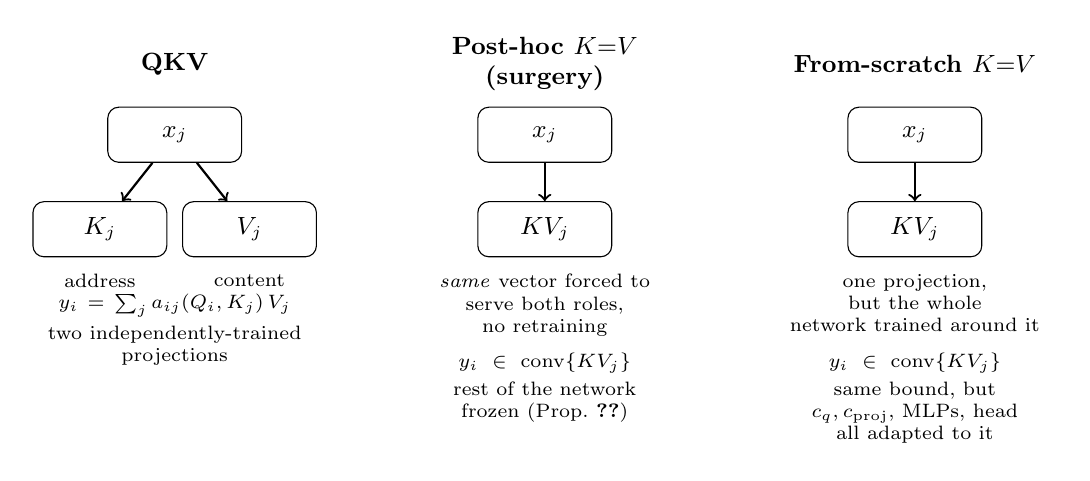
\begin{tikzpicture}[
  box/.style={draw, rounded corners, minimum width=1.7cm, minimum height=0.7cm, align=center, font=\small},
  lbl/.style={font=\scriptsize, align=center, text width=3.5cm},
  arr/.style={->, thick}
]
\node[font=\small\bfseries] (t1) at (0,2.7) {QKV};
\node[box] (x1) at (0,1.8) {$x_j$};
\node[box] (k1) at (-0.95,0.6) {$K_j$};
\node[box] (v1) at (0.95,0.6) {$V_j$};
\node[lbl,text width=1.2cm,anchor=north] at (-0.95,0.15) {address};
\node[lbl,text width=1.2cm,anchor=north] at (0.95,0.15) {content};
\draw[arr] (x1) -- (k1);
\draw[arr] (x1) -- (v1);
\node[lbl,anchor=north] at (0,-0.1) {$y_i=\sum_j a_{ij}(Q_i,K_j)\,V_j$\\[2pt] two independently-trained\\ projections};

\node[font=\small\bfseries, align=center] (t2) at (4.7,2.7) {Post-hoc $K{=}V$\\(surgery)};
\node[box] (x2) at (4.7,1.8) {$x_j$};
\node[box] (kv2) at (4.7,0.6) {$KV_j$};
\node[lbl,anchor=north] at (4.7,0.15) {\emph{same} vector forced to\\serve both roles, no retraining};
\draw[arr] (x2) -- (kv2);
\node[lbl,anchor=north] at (4.7,-0.85) {$y_i \in \mathrm{conv}\{KV_j\}$\\[2pt] rest of the network frozen (Prop.~\ref{prop:hull})};

\node[font=\small\bfseries, align=center] (t3) at (9.4,2.7) {From-scratch $K{=}V$};
\node[box] (x3) at (9.4,1.8) {$x_j$};
\node[box] (kv3) at (9.4,0.6) {$KV_j$};
\node[lbl,anchor=north] at (9.4,0.15) {one projection, but the whole\\network trained around it};
\draw[arr] (x3) -- (kv3);
\node[lbl,anchor=north] at (9.4,-0.85) {$y_i \in \mathrm{conv}\{KV_j\}$\\[2pt] same bound, but $c_q,c_{\text{proj}}$, MLPs, head all adapted to it};
\end{tikzpicture}
\caption{The same architecture, $K{=}V$, reached two different ways. Left: the QKV
teacher, with independent $K$/$V$ projections free to specialize for addressing and
content separately. Middle: post-hoc surgery forces one already-specialized
representation to do both jobs, with nothing else in the network adjusted
(Section~\ref{sec:mechanism} finds the result closer to a basis mismatch than to
information loss). Right: choosing $K{=}V$ \emph{before} training lets every other
parameter co-adapt to it from the start -- the same mathematical bound
(Proposition~\ref{prop:hull}) applies, but nothing has to unlearn a different
assumption.}
\label{fig:concept}
\end{figure}

\section{A convex-hull obstruction}
\label{sec:hull}

\begin{proposition}[Convex-hull confinement under K=V]
\label{prop:hull}
If $k_j = v_j$ for every position $j$ (as holds for all three surgery modes above,
and for the from-scratch \texttt{Q=K=V} and \texttt{Q}$\neq$\texttt{K=V} variants),
then for every query position $i$,
\[
y_i \in \operatorname{conv}\{k_1, \dots, k_T\} \subseteq \operatorname{span}\{k_1,
\dots, k_T\},
\]
regardless of the attention weights $a_{ij}$.
\end{proposition}
\begin{proof}
$a_{ij} \geq 0$ and $\sum_j a_{ij} = 1$ by construction of the softmax, so $y_i =
\sum_j a_{ij} k_j$ is by definition a convex combination of $\{k_j\}$.
\end{proof}

\begin{corollary}
\label{cor:content}
The attention sub-block can only make available to position $i$ information that is
already representable inside $\operatorname{span}\{k_1,\dots,k_T\}$. If the trained
$K$-projection was shaped by gradient descent to produce a good \emph{addressing}
signal ($q_i \cdot k_j$ ranking the correct target highest) without pressure to remain
\emph{injective} in the token content $x_j$ --- because that pressure was carried
entirely by the independent $V$-projection in the QKV teacher --- then $k_j$ need not
determine $x_j$, and routing $k_j$ itself to position $i$ can lose the very content
the downstream task needs. This is a hypothesis about \emph{why} surgery hurts, stated
here before we test it; Section~\ref{sec:mechanism} probes addressing and content
recoverability directly and finds the picture is more specific than ``$K$ lacks
content'' as stated -- content is present in $K$ too, but evidently in a form the rest
of the network cannot use.
\end{corollary}

\begin{remark}[Invariance to normalization]
\label{rem:norm}
Proposition~\ref{prop:hull}'s proof uses only that $a_{ij}\ge 0$ and $\sum_j a_{ij}=1$;
it places no assumption on how $k_j$ (equivalently $v_j$, since $k_j=v_j$) is
computed. It therefore holds unchanged whether $k_j$ is a raw linear projection, an
$\ell_2$-normalized projection (as in QK-normalized attention variants), or the output
of any other fixed transformation applied before the weighted sum -- confinement is to
the convex hull of whatever vectors are actually summed, in whatever geometry they
live in. In the checkpoints studied here, LayerNorm is applied pre-block to the
residual stream $x_j$ before $c_k, c_v$ project it (Section~\ref{sec:setup}), not to
$k_j$ or $v_j$ themselves, so this is a non-issue for our experiments specifically; we
state the general invariance here because it is easy to construct architectures where
it would otherwise look like a threat to the argument. A normalization that discarded
information $v_j$ needed to retain would show up as a smaller effective
$\operatorname{span}\{k_j\}$ in Corollary~\ref{cor:content}'s premise, not as a failure
of Proposition~\ref{prop:hull} itself, which is unconditional.
\end{remark}

\begin{remark}[Scope: one attention sub-block, not the whole transformer]
\label{rem:scope}
Proposition~\ref{prop:hull} constrains $y_i$, the output of one attention sub-block.
It does not constrain $h_i^{\text{out}} = h_i^{\text{in}} + y_i$, the MLP applied to
it, or any later layer: the residual stream carries $h_i^{\text{in}}$ forward
regardless of what the attention sub-block computes, and nothing here restricts what
a downstream MLP or a later attention layer (with its own, unconstrained $K'/V'$) can
do with the result. A model with $K=V$ in every layer is therefore \emph{not}
restricted to representing only what lies in a single layer's convex hull -- claiming
that would be a claim about the whole network's expressivity, which Proposition~
\ref{prop:hull} does not make and we do not intend. What the proposition does say is
narrower and, we think, still useful: a single $K=V$ attention operation cannot
independently choose the representation used for content transport from the
representation used for addressing -- what gets transported to position $i$ must be a
convex combination of the very vectors $\{k_j\}$ that determined \emph{where} to look,
not some separately-chosen payload. Whether that narrower constraint ends up
mattering for a given task is exactly the empirical question the rest of the note is
about.
\end{remark}

Proposition~\ref{prop:hull} is therefore silent on \emph{when} its obstruction
actually bites in practice: a task that never needs cross-token content routing in
the first place is immune to it regardless of how many layers have $K=V$.
Section~\ref{sec:pointwise} makes this precise for our tasks; Section~\ref{sec:empirical}
shows that even among the routing-dependent tasks, the practical severity varies with
how much the teacher's $K$ and $V$ projections had actually specialized
(Corollary~\ref{cor:content}'s premise) -- which we measure and test directly rather
than assume, and which turns out to need a more specific account than the corollary as
originally stated (Section~\ref{sec:mechanism}).

\section{Why pointwise tasks are immune}
\label{sec:pointwise}

Two of the five synthetic tasks are pointwise: \textsc{sub} computes $y_i = 9 - x_i$
and \textsc{copy} computes $y_i = x_i$, each a function of position $i$'s own input
only. Each block's residual connection preserves a direct, additive path from
position $i$'s own incoming representation ($\text{embed}(x_i) + \text{pos\_emb}(i)$
at the first block, that block's own input thereafter) through to its output,
regardless of what the attention sub-block computes; stacked over every block, that
representation is never overwritten, only added to. Combined with per-position MLPs
that are already universal approximators of pointwise maps, attention's specific
content-routing is therefore not load-bearing for these two tasks, and
Proposition~\ref{prop:hull}'s obstruction is vacuous: it restricts what attention can
contribute, but the task does not need attention to contribute anything.

This is not merely a plausibility argument -- it is directly testable with data we
already have. If attention's specific query--key matching mattered for \textsc{sub}/
\textsc{copy}, corrupting the value stream with either the wrong projection
(\textsc{keep\_k}) or corrupting the key stream with the wrong projection
(\textsc{keep\_v}) should hurt \emph{at least one} of the two directions. Instead,
Table~\ref{tab:synthetic} shows \emph{both} surgeries leave \textsc{sub} and
\textsc{copy} at $1.000$ accuracy, exactly as the residual-bypass account predicts,
while the three routing-dependent tasks (\textsc{reverse}, \textsc{sort},
\textsc{swap} -- each requires moving a \emph{different} position's value to position
$i$) collapse sharply under the same surgeries.

\section{Empirical validation}
\label{sec:empirical}

\subsection{Zero-shot surgery and distillation recovery}

Table~\ref{tab:synthetic} and Table~\ref{tab:vision} report, for each task/dataset:
the from-scratch \texttt{QKV} teacher accuracy, the from-scratch tied
(\texttt{Q}$\neq$\texttt{K=V}) baseline accuracy (a reference performance a distilled
student can reasonably target -- not a hard ceiling, since \textsc{avg}/CIFAR-10
slightly exceeds it (see Table~\ref{tab:vision})), the zero-shot accuracy immediately
after surgery (no fine-tuning), and the accuracy after
5 epochs of distillation from the QKV teacher (cross-entropy on hard labels + KL
divergence against the teacher's soft logits, $T=2$, equal weighting).

\begin{table}[h]
\centering
\small
\begin{tabular}{llccccc}
\toprule
Task & Mode & QKV & Q$\neq$K=V (scratch) & Zero-shot surgery & Distilled (5 ep) \\
\midrule
REVERSE & keep\_k & 1.000 & 1.000 & 0.100 & 1.000 \\
        & keep\_v & 1.000 & 1.000 & 0.123 & 1.000 \\
        & avg     & 1.000 & 1.000 & 0.861 & 1.000 \\
SORT    & keep\_k & 0.998 & 0.996 & 0.583 & 0.965 \\
        & keep\_v & 0.998 & 0.996 & 0.717 & 0.996 \\
        & avg     & 0.998 & 0.996 & 0.751 & 0.996 \\
SUB     & any     & 1.000 & 1.000 & 1.000 & 1.000 \\
SWAP    & keep\_k & 1.000 & 1.000 & 0.088 & 1.000 \\
        & keep\_v & 1.000 & 1.000 & 0.122 & 1.000 \\
        & avg     & 1.000 & 1.000 & 0.906 & 1.000 \\
COPY    & any     & 1.000 & 1.000 & 1.000 & 1.000 \\
\bottomrule
\end{tabular}
\caption{Synthetic sequence tasks (token accuracy). Routing-dependent tasks
(REVERSE, SORT, SWAP) collapse under surgery and recover under distillation;
pointwise tasks (SUB, COPY) are unaffected by either. 14 of these 15 (task,
surgery-mode) configurations reach the from-scratch tied baseline within 5 epochs; the one
exception, SORT/\textsc{keep\_k}, reaches 0.965 against a 0.996 target and is still
improving at epoch 5.}
\label{tab:synthetic}
\end{table}

\begin{table}[h]
\centering
\small
\resizebox{\textwidth}{!}{%
\begin{tabular}{llcccccc}
\toprule
Dataset & Mode & QKV & Q$\neq$K=V (scratch) & Zero-shot surgery & Distilled (5 ep) & Distilled (10 ep) \\
\midrule
MNIST     & keep\_k & 0.981 & 0.978 & 0.114 & 0.979 & -- \\
          & keep\_v & 0.981 & 0.978 & 0.151 & 0.982 & -- \\
          & avg     & 0.981 & 0.978 & 0.910 & 0.983 & -- \\
FMNIST    & keep\_k & 0.887 & 0.882 & 0.084 & 0.881 & -- \\
          & keep\_v & 0.887 & 0.882 & 0.105 & 0.883 & -- \\
          & avg     & 0.887 & 0.882 & 0.811 & 0.888 & -- \\
CIFAR-10  & keep\_k & 0.696 & 0.698 & 0.076 & 0.631 & 0.666 \\
          & keep\_v & 0.696 & 0.698 & 0.153 & 0.686 & 0.693 \\
          & avg     & 0.696 & 0.698 & 0.368 & 0.696 & \textbf{0.702} \\
CIFAR-100 & keep\_k & 0.437 & 0.445 & 0.007 & 0.384 & 0.411 \\
          & keep\_v & 0.437 & 0.445 & 0.021 & 0.424 & 0.430 \\
          & avg     & 0.437 & 0.445 & 0.109 & 0.432 & 0.435 \\
\bottomrule
\end{tabular}%
}
\caption{Vision classification (ViT, top-1 accuracy). Unlike the synthetic tasks,
every dataset shows some collapse under \textsc{keep\_k}/\textsc{keep\_v}: these ViTs
classify from a learned \textsc{cls} token (\texttt{h[:, 0]} after the final block),
not global average pooling, so which patches reach the classification decision is
itself an attention-weighted, content-routing operation rather than a fixed uniform
average -- there is no pointwise bypass analogous to Section~\ref{sec:pointwise}. At
the 5-epoch budget, \textsc{keep\_k} on CIFAR-10 and
CIFAR-100 was still visibly improving, so both CIFAR datasets (all three modes) were
rerun with a 10-epoch budget; MNIST/FMNIST were not rerun since they were already
converged by 5 epochs. \textsc{keep\_v} and \textsc{avg} are essentially converged on
CIFAR by 10 epochs (\textsc{avg}/CIFAR-10 slightly exceeds the from-scratch tied baseline);
\textsc{keep\_k} closes only about half its remaining gap, and its per-epoch curve is
already plateauing by epoch 8--9 (full curves in
\texttt{distillation\_vision\_cifar\{10,100\}\_10ep.csv}), indicating a genuinely
harder, slower-converging recovery rather than simple under-training at 5 epochs.}
\label{tab:vision}
\end{table}

\textsc{avg} is uniformly the safer zero-shot surgery on every vision dataset, and
doubling the distillation budget does not treat all three surgery modes equally:
\textsc{keep\_k} is the one mode with a persistent gap even at 10 epochs (Section~
\ref{sec:mechanism} tests why, on the synthetic tasks, and finds the evidence more
consistent with a basis-mismatch account than a simple content-loss one).

Tables~\ref{tab:synthetic}--\ref{tab:vision} report only endpoint accuracies;
Figure~\ref{fig:curves} shows the full per-epoch recovery curve for every (task or
dataset, surgery-mode) configuration referenced above. The shape confirms what the
endpoints suggest: REVERSE/SUB/SWAP/COPY and MNIST are already flat by epoch 1 (the
surgery was mild or the gap closes almost immediately), SORT/\textsc{keep\_k} and every
CIFAR/\textsc{keep\_k} curve are still rising through their full epoch budget without
having visibly plateaued as early as epoch 2--3, and \textsc{keep\_v}/\textsc{avg} on
CIFAR flatten out well before their budget ends -- consistent with \textsc{keep\_k}
being a harder optimization problem rather than merely a deeper hole to climb out of.

\begin{figure}[h]
\centering
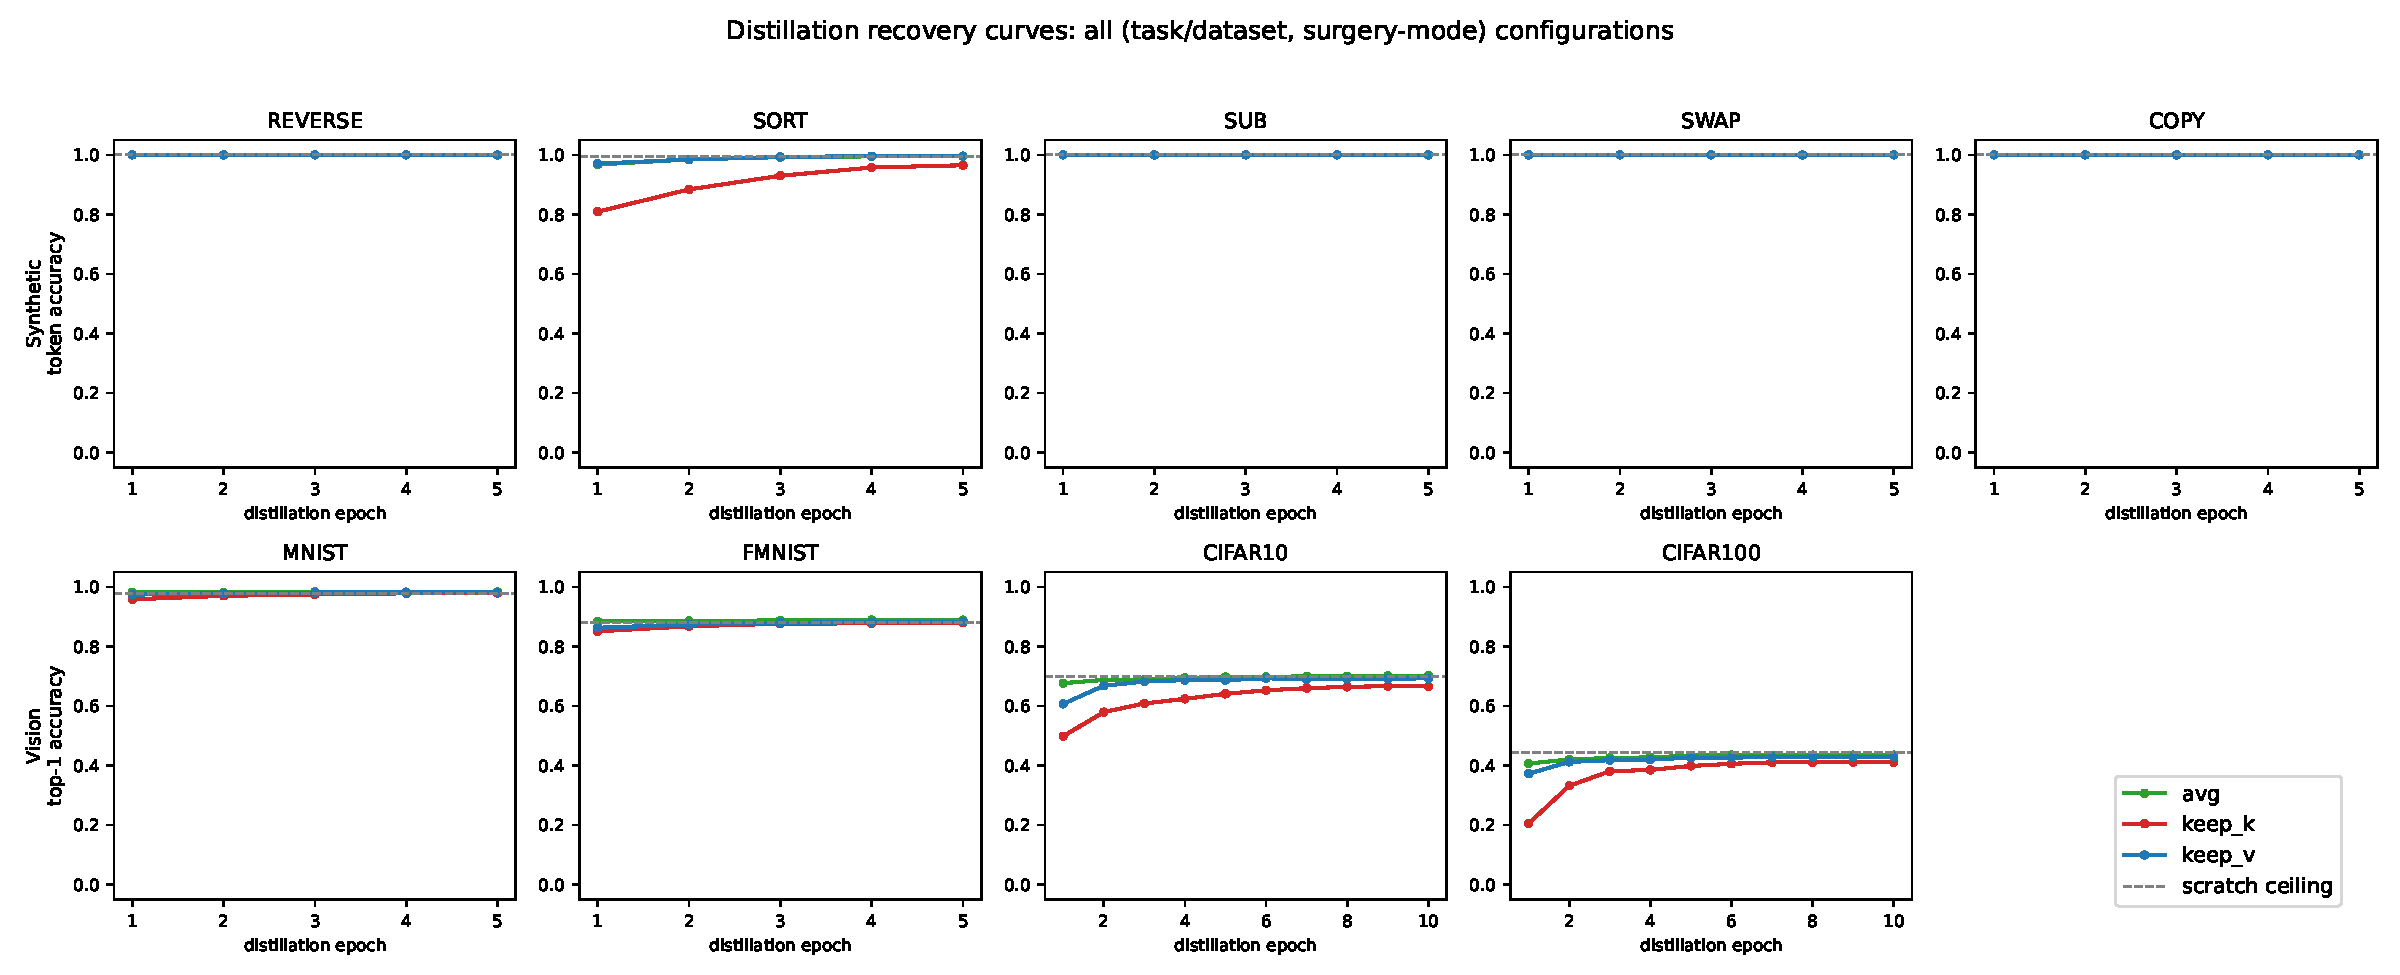
\includegraphics[width=\textwidth]{../distillation_curves_full.pdf}
\caption{Per-epoch distillation accuracy for every (task/dataset, surgery-mode)
configuration in Tables~\ref{tab:synthetic}--\ref{tab:vision} (dashed line: the
from-scratch Q$\neq$K=V tied baseline). CIFAR-10/CIFAR-100 panels show the full 10-epoch
runs; all other panels are the 5-epoch runs (not rerun longer since already
converged).}
\label{fig:curves}
\end{figure}

\textbf{Where does the zero-shot optimum sit, and is reusing $K$ better than noise?}
Tables~\ref{tab:synthetic}--\ref{tab:vision} report only three points along the line
$c_{kv} = \alpha W_K + (1-\alpha) W_V$ ($\alpha{=}1$: \textsc{keep\_k}, $\alpha{=}0$:
\textsc{keep\_v}, $\alpha{=}0.5$: \textsc{avg}). Figure~\ref{fig:alpha} sweeps
$\alpha \in \{0, 0.1, \dots, 1.0\}$ and adds a fourth reference point: $c_{kv}$ left at
its fresh, untrained initialization, with no relationship to the teacher's $K$ or $V$
at all -- reported as a mean $\pm$ 1 std.\ over 5 random seeds, not a single number,
since the baseline's own sampling variance turns out to matter for what we can claim
about it.

Two things stand out. First, the curve is neither monotonic nor symmetric around
\textsc{avg}: REVERSE, SWAP, and all four vision datasets peak near
$\alpha \approx 0.4$--$0.5$, while SORT peaks earlier, around $\alpha \approx 0.2$--
$0.3$, and degrades monotonically from there to \textsc{keep\_k}. SUB and COPY are
flat at $1.000$ across every $\alpha$, including every random seed -- a stronger
confirmation of Section~\ref{sec:pointwise} than the three original discrete points.

Second: \textsc{keep\_k} does not reliably preserve useful downstream functionality
despite preserving linearly decodable content (Section~\ref{sec:mechanism}). Table~
\ref{tab:randombaseline} compares \textsc{keep\_k} against the random baseline's mean
and std.\ for each non-pointwise task. On SWAP, \textsc{keep\_k} sits about 12 random-
baseline standard deviations below the mean -- unambiguous. On the other five
(REVERSE, SORT, MNIST, FMNIST, CIFAR-10, CIFAR-100), \textsc{keep\_k} sits within
about 2 standard deviations of the random baseline in either direction, which at
$n=5$ seeds we cannot call a reliable difference from noise in either direction. We
had originally read the point estimates alone as ``\textsc{keep\_k} is usually at or
below random,'' which overstated what 5 seeds actually support; the defensible claim
is narrower and, we think, still the interesting one: outside of SWAP's dramatic case,
\textsc{keep\_k}'s specialized (non-random) $K$-derived representation confers no
detectable advantage over uninformative noise to the frozen downstream network, even
though Section~\ref{sec:mechanism}'s probe shows that representation is just as
linearly content-rich as $V$'s.

\begin{figure}[h]
\centering
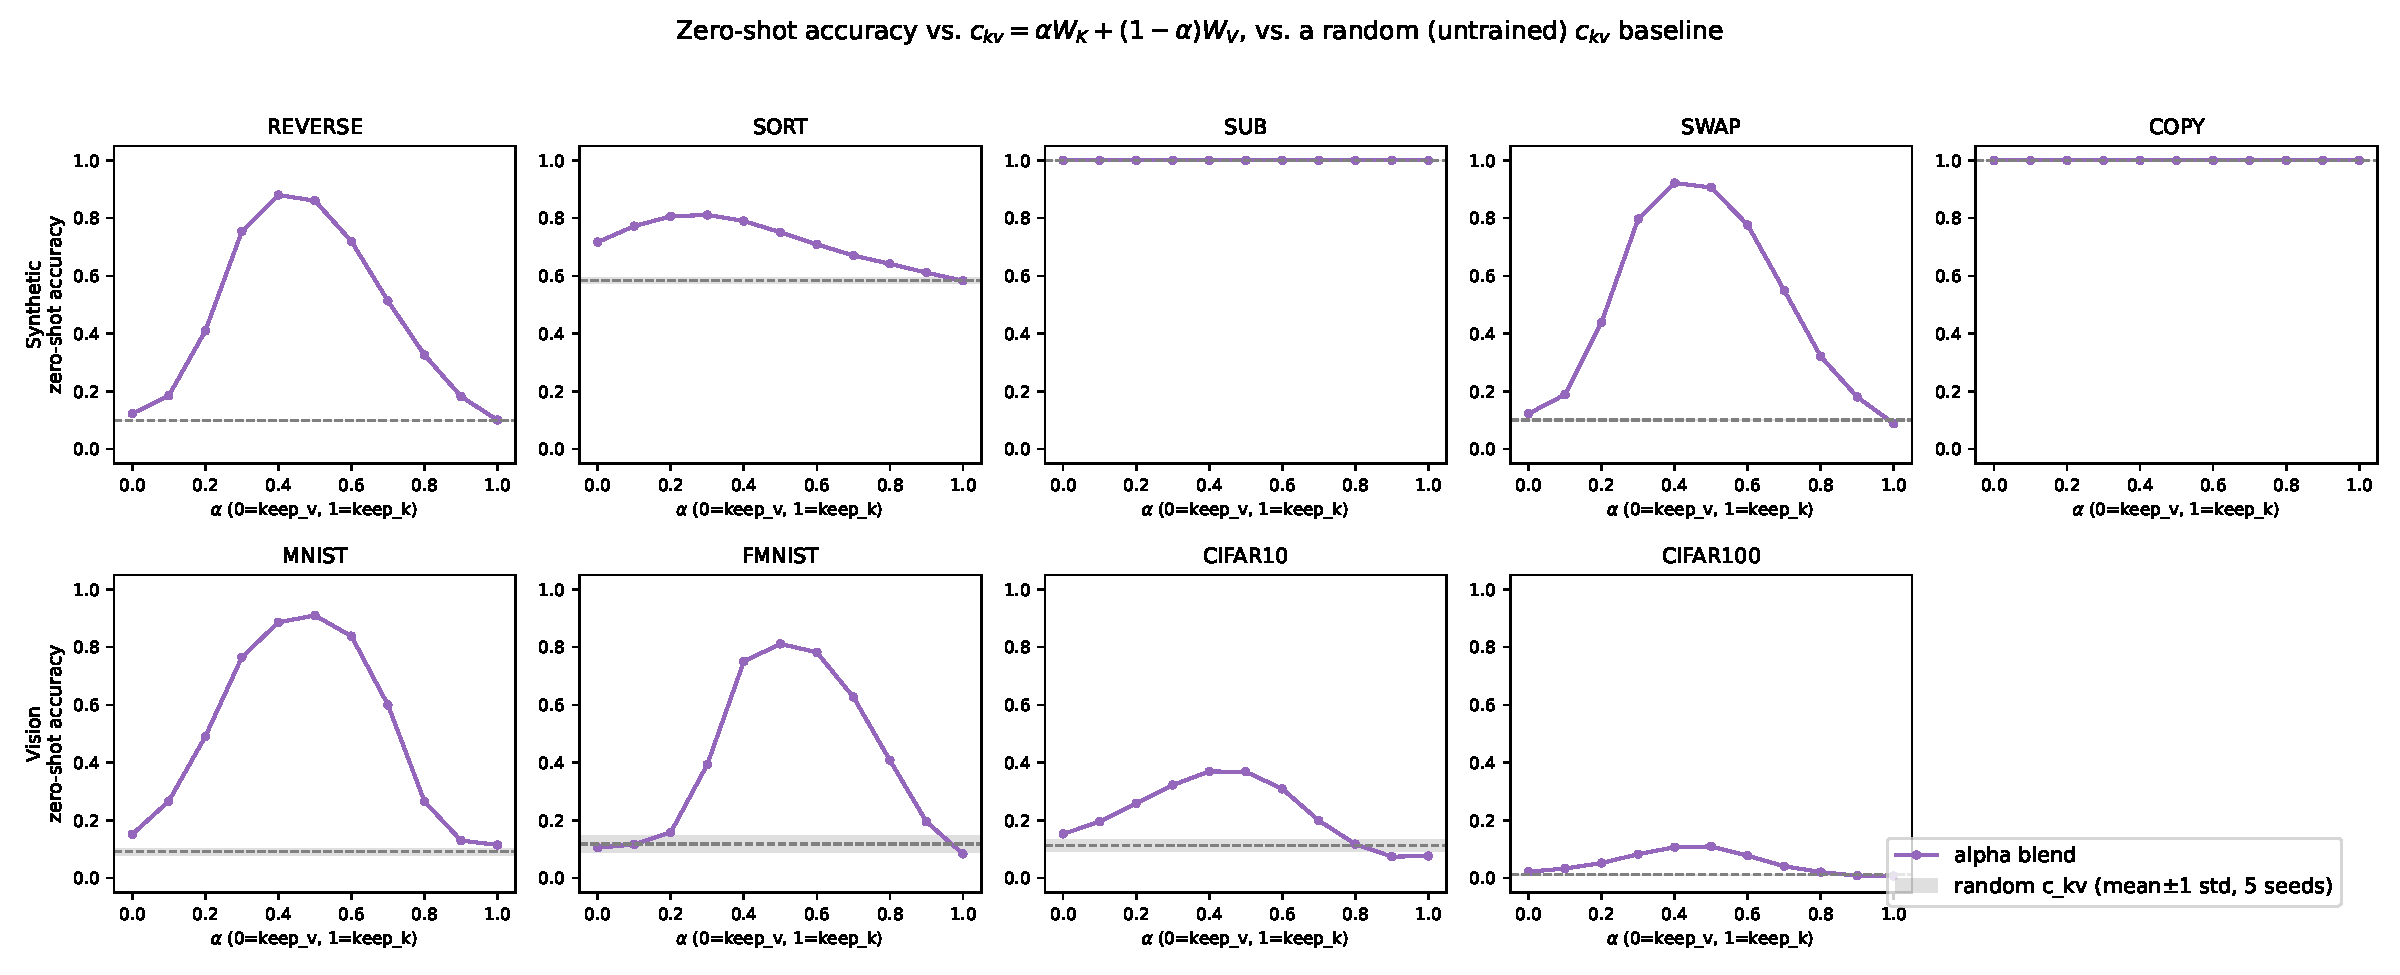
\includegraphics[width=\textwidth]{../kv_alpha_sweep.pdf}
\caption{Zero-shot accuracy as $c_{kv}$ is swept from \textsc{keep\_v}
($\alpha{=}0$) to \textsc{keep\_k}
($\alpha{=}1$), vs.\ a random-initialization $c_{kv}$ baseline (shaded: mean $\pm$ 1
std.\ over 5 seeds). No retraining anywhere in this figure.}
\label{fig:alpha}
\end{figure}

\begin{table}[h]
\centering
\small
\begin{tabular}{lccc}
\toprule
Task/dataset & \textsc{keep\_k} & random $c_{kv}$ (mean $\pm$ std, 5 seeds) & $z$ \\
\midrule
REVERSE   & 0.100 & $0.100 \pm 0.0004$ & $+1.25$ \\
SORT      & 0.583 & $0.584 \pm 0.0099$ & $-0.12$ \\
SWAP      & 0.088 & $0.100 \pm 0.0010$ & $-12.30$ \\
MNIST     & 0.114 & $0.091 \pm 0.0124$ & $+1.92$ \\
FMNIST    & 0.084 & $0.118 \pm 0.0278$ & $-1.23$ \\
CIFAR-10  & 0.076 & $0.112 \pm 0.0210$ & $-1.72$ \\
CIFAR-100 & 0.007 & $0.011 \pm 0.0024$ & $-1.88$ \\
\bottomrule
\end{tabular}
\caption{\textsc{keep\_k} vs.\ the random-$c_{kv}$ baseline, with $z = (\text{keep\_k}
- \text{mean})/\text{std}$. Only SWAP is a large, unambiguous effect; the rest are
within about 2 standard deviations of the random baseline's own spread at $n=5$
seeds, i.e.\ not reliably distinguishable from noise in either direction. SUB and
COPY are omitted: every mode, including all 5 random seeds, scores exactly $1.000$.}
\label{tab:randombaseline}
\end{table}

\textbf{Confirmation at language-model scale.} Everything above uses small models
(1--2M-param vision ViTs, tiny sequence models) where a full $\alpha$-sweep and a
5-seed random baseline are cheap. To check the collapse-and-recover pattern at a scale closer
to production LLM pretraining, we repeat the core protocol -- QKV teacher, surgical
tying, zero-shot eval, distillation recovery -- on the base paper's 300M-parameter
GPT-style model, trained from scratch on 10B tokens of FineWeb-Edu
(\texttt{outputs\_qkv\_baseline\_10B/final\_model.pt}, validation perplexity 20.82),
against the base paper's matching from-scratch \texttt{Q}$\neq$\texttt{K=V} checkpoint
(perplexity 21.28) as the tied ceiling. Distillation uses the same
hard-label-CE + KL-vs.-teacher-soft-logits objective ($T{=}2$, equal weighting) as
Tables~\ref{tab:synthetic}--\ref{tab:vision}, but for a 500M-token budget (about 5\% of
the from-scratch pretraining budget, in the same spirit as the epoch budgets used
above) rather than a fixed epoch count, since ``epoch'' is not a meaningful unit
against a pretraining corpus far larger than the distillation budget itself.

\begin{table}[h]
\centering
\small
\begin{tabular}{lcccc}
\toprule
Mode & QKV teacher & Q$\neq$K=V (scratch) & Zero-shot surgery & Distilled (500M tok) \\
\midrule
keep\_k & 20.82 & 21.28 & 13345.19 & 29.00 \\
keep\_v & 20.82 & 21.28 & 7347.14  & 27.00 \\
avg     & 20.82 & 21.28 & 6430.36  & 22.87 \\
\bottomrule
\end{tabular}
\caption{FineWeb-Edu language modeling (300M params, validation perplexity --
lower is better, unlike the accuracy tables above). Causal next-token prediction is
not a pointwise task in the sense of Section~\ref{sec:pointwise}: every position's
prediction depends on routing information forward from earlier tokens, so
Proposition~\ref{prop:hull} predicts collapse under $K=V$ tying, and zero-shot surgery
confirms it dramatically -- perplexity worsens by two to three orders of magnitude
(20.8 $\to$ 6{,}400--13{,}300) versus the roughly one-order-of-magnitude accuracy
collapses in Tables~\ref{tab:synthetic}--\ref{tab:vision}, consistent with
perplexity's exponential sensitivity to per-token log-loss rather than a qualitatively
different failure mode. Distillation recovers all three modes to within 1.6--7.7
perplexity points of the scratch-tied ceiling (\textsc{avg} closest, \textsc{keep\_k}
furthest), reproducing the same
\textsc{avg}~$>$~\textsc{keep\_v}~$>$~\textsc{keep\_k} ordering, by both zero-shot
severity and post-distillation gap, seen in Table~\ref{tab:vision}.}
\label{tab:llm}
\end{table}

The ranking replicates exactly. \textsc{avg} is again the safest zero-shot surgery and
recovers closest to the tied ceiling (22.87 vs.\ 21.28, a 1.6-point gap after 500M
distillation tokens), echoing \textsc{avg}/CIFAR-10's near-complete recovery in
Table~\ref{tab:vision}; \textsc{keep\_k} is again both the worst zero-shot mode and the
one with the largest residual gap after distillation (29.00 vs.\ 21.28), matching the
persistent \textsc{keep\_k} gap already seen at vision scale (Section~
\ref{sec:discussion}). The teacher's $K$/$V$ activation CKA -- cheap to measure, since
it needs only a forward pass on held-out data and no retraining -- is $0.70$, squarely
inside the range spanned by the 9 synthetic/vision teachers. Converting perplexity to a
chance-normalized log-loss severity (Figure~\ref{fig:cka}'s caption gives the exact
transform) places the LLM point within the same scatter around Figure~\ref{fig:cka}'s
$n=9$ fit line as the other 9 points (residual $0.19$, in the same range as, e.g.,
\textsc{fmnist}'s $0.14$ or REVERSE's $0.25$) despite not being part of it -- consistent
with, though not a tight confirmation of, the CKA--severity relationship extending to a
domain and scale neither of the original 9 points covers. We do not fold it into that
figure's $r=-0.84$ correlation regardless, since the normalization is a different
derivation from the other 9 points' raw accuracy drop, not a validated equivalent
measure.

A cheap, no-retraining content probe (same closed-form ridge-regression method as
Section~\ref{sec:mechanism}, adapted for the 50{,}304-token vocabulary via an
index-add accumulation in place of a dense one-hot target matrix, and with the ridge
penalty scaled to the data's own diagonal energy rather than a fixed constant --
this model's $K$/$V$ activations turn out to be severely rank-deficient, and a fixed
ridge silently degenerates the closed-form solve into float32 noise at one layer if
left unscaled) tells a different story from the synthetic/vision result, though.
Averaged over the model's 20 layers, the probe recovers token identity from $v_j$
noticeably better than from $k_j$ ($85.3\%$ vs.\ $80.3\%$ mean accuracy, a $5.0$-point
gap on average, ranging from $1.7$ to $10.9$ points across layers, with $V$ ahead at
every single one -- full per-layer numbers in
\texttt{kv\_content\_probe\_llm\_results.csv}). At synthetic/vision scale, $K$ and $V$
probed equally well, which is precisely what motivated moving away from
Corollary~\ref{cor:content}'s original content-loss story toward the basis-mismatch
account (Section~\ref{sec:mechanism}). Here, the LLM teacher's $K$ \emph{is}
measurably harder to decode token identity from than $V$ -- closer to
Corollary~\ref{cor:content} as originally stated. We read this as a genuine point of
divergence rather than force it into the existing account: the gap is consistent in
direction across every layer, but modest in size (both projections still probe well
above 80\%), so it does not on its own settle whether basis-mismatch, partial
content-loss, or both is the better description at this scale -- and, like the other
single-point checks in this section, it comes from one held-out batch, not a
bootstrapped or multi-seed estimate.

We did not repeat the $\alpha$-sweep or random-$c_{kv}$ baseline
(Section~\ref{sec:mechanism} onward) at this scale -- each would cost a multi-GPU-day
training run per point here rather than the few seconds it takes at vision/synthetic
scale -- so this result is best read as a
single confirmatory data point on the headline collapse-and-recover pattern, not a
full replication of the mechanistic analysis.

\subsection{Testing the addressing/content mechanism directly}
\label{sec:mechanism}

Corollary~\ref{cor:content} rests on an assumption we had not, until now, tested
directly: that the teacher's $K$-projection specialized for \emph{addressing} at some
cost to \emph{content}, while $V$ specialized the other way. We test both halves on
the five synthetic-task teachers, where the correct routing target at each position
is known exactly (COPY/SUB: self; REVERSE: position $T{-}1{-}i$; SWAP: swap the two
halves; SORT: the source position is $\arg\mathrm{sort}(x)$, which is per-sample and
data-dependent).

\textbf{Addressing.} For each layer, we take the model's actual attention weights
$a_{ij}$ (re-derived from the true layer-normed block input via a forward hook, not
recomputed independently) and check whether $\arg\max_j a_{ij}$ matches the
task's ground-truth source position. On the two genuinely one-to-one permutation
tasks this is strong (REVERSE $1.00 \to 0.83$ from layer 0 to 1; SWAP $1.00 \to
0.78$). On SUB and COPY it is near chance ($\approx 0.02$--$0.05$) at both layers,
consistent with Section~\ref{sec:pointwise}: attention apparently does not implement
self-addressing for these, because it does not need to. SORT is \emph{also} near
chance under this diagnostic, which we do not read as evidence against SORT needing
routing -- it collapses under surgery just like REVERSE/SWAP (Table~\ref{tab:synthetic})
-- but as a sign that ``does argmax match one ground-truth index'' is the wrong
operationalization for a task whose natural solution is a distributed rank/comparison
computation over many positions rather than a hard one-to-one copy. We report this as
a limitation of the diagnostic, not a finding about SORT's mechanism.

\textbf{Content.} We fit a closed-form ridge-regression linear probe from $k_j$
(resp.\ $v_j$) to $x_j$'s one-hot identity, on a held-out train/test split, and report
test-set classification accuracy. The result complicates Corollary~\ref{cor:content}
as stated: at this model's width ($d{=}256$), \emph{both} $k_j$ and $v_j$ probe at or
near $1.000$ on every task and both layers, with no consistent gap (the one partial
exception, SORT layer 1, is $1.000$ for $K$ vs.\ $0.991$ for $V$ -- if anything the
wrong direction for the hypothesis). So the teacher's $K$-projection has not, in any
sense a linear probe can detect, sacrificed the ability to reconstruct token
identity. Corollary~\ref{cor:content}'s premise -- that $K$ is under no pressure to
stay content-decodable -- does not hold as a loss of \emph{linearly available
information}, at least not at this scale.

Read together with the alpha-sweep/random-baseline result above, this points to a
more specific mechanism than ``$K$ lost the content'': \textsc{keep\_k} confers no
detectable advantage over an untrained random baseline on most non-pointwise tasks,
and is dramatically worse on one (SWAP; Table~\ref{tab:randombaseline}), even though
$k_j$ is linearly just as decodable as $v_j$. $K$ does not reliably preserve useful
downstream functionality despite preserving content, which is consistent with a
\textbf{basis mismatch} rather than an information loss -- though we have not
measured downstream calibration to $K$ vs.\ $V$ directly, so we hold this as the
best-supported reading rather than an established mechanism: $k_j$ carries $x_j$'s
identity in a representation shaped by the addressing objective ($q_i \cdot k_j$
ranking correctly), not in the representation $c_{\text{proj}}$, the MLP, and the head
were calibrated against -- and handing those frozen downstream weights an unfamiliar
(if information-rich) basis is, on the evidence in Table~\ref{tab:randombaseline}, no
more useful to them than noise. We did not anticipate this when
first writing Corollary~\ref{cor:content}, and we think it is a more precise and more
interesting claim than the one we originally set out to test -- and it is also
consistent with why distillation recovers \textsc{keep\_k} slowest
(Section~\ref{sec:discussion}): re-calibrating a frozen network to a new, unfamiliar
basis is a harder fitting problem than recovering from noise-level information loss
would be.

\subsection{Two direct tests of the basis-mismatch account}
\label{sec:direct-tests}

Everything above is indirect evidence for basis mismatch: a probe showing content
survives, a random baseline showing that content is nonetheless useless, a
distillation-speed asymmetry consistent with re-calibration being the bottleneck.
None of it manipulates the hypothesized mechanism directly. We add two zero-shot
(no retraining) experiments that do: separately vary which projection produces
attention \emph{scores} versus which produces the \emph{transported} vectors, and
directly correct $K$'s basis toward $V$'s with a learned map fit on held-out data.

\textbf{Addressing/payload decomposition.} Writing $A(S, P)$ for attention with
scores from $S$ and transported payload from $P$, the teacher computes $A(Q,K)V$ and
there are three other cells: $A(Q,K)K$, $A(Q,V)V$, $A(Q,V)K$. Two of these are not
new experiments -- they are exactly what \textsc{keep\_k}/\textsc{keep\_v} already
measured: tying $c_{kv} \leftarrow c_k$ reuses $c_k$ for \emph{both} roles, so
scores are unchanged ($A(Q,K)$) and the payload becomes $K$; symmetrically for
\textsc{keep\_v} and $c_v$. Only $A(Q,V)K$ -- scores from $V$, payload from $K$ --
is genuinely new. We evaluate it by monkey-patching the teacher's own attention
forward (no new model, no retraining), on the same held-out data as
Tables~\ref{tab:synthetic}--\ref{tab:vision}.

\begin{table}[h]
\centering
\small
\begin{tabular}{lcccc}
\toprule
Task/dataset & $A(Q,K)V$ (teacher) & $A(Q,K)K$ (\textsc{keep\_k}) & $A(Q,V)V$ (\textsc{keep\_v}) & $A(Q,V)K$ (new) \\
\midrule
REVERSE   & 1.000 & 0.100 & 0.123 & 0.104 \\
SORT      & 0.998 & 0.583 & 0.717 & 0.576 \\
SWAP      & 1.000 & 0.088 & 0.122 & 0.108 \\
MNIST     & 0.981 & 0.114 & 0.151 & 0.081 \\
FMNIST    & 0.887 & 0.084 & 0.105 & 0.099 \\
CIFAR-10  & 0.696 & 0.076 & 0.153 & 0.073 \\
CIFAR-100 & 0.437 & 0.007 & 0.021 & 0.006 \\
\bottomrule
\end{tabular}
\caption{Addressing/payload decomposition, zero-shot accuracy (SUB/COPY omitted:
$1.000$ in every cell, as always). $A(Q,V)K$ tracks $A(Q,K)K$ (\textsc{keep\_k})
closely on SORT and both CIFAR datasets -- evidence that \emph{payload} identity,
not addressing identity, drives the damage there, directly supporting the
basis-mismatch reading of \textsc{keep\_k}'s failure. REVERSE, SWAP, and MNIST
instead collapse to a similar floor regardless of the combination, consistent with
these one-to-one-routing tasks being sensitive to any deviation from the exact
trained pairing.}
\label{tab:decomposition}
\end{table}

At LLM scale the same swap gives val.\ PPL $9622.90$ for $A(Q,V)K$ -- between
\textsc{keep\_k} ($13345.19$) and \textsc{keep\_v} ($7347.14$), mildly closer to
\textsc{keep\_v}, i.e.\ a less clean "payload dominates" signal than SORT/CIFAR
show. We read this as a genuine, honestly-reported scale-dependence rather than
force one story onto both: at small scale payload identity is often the dominant
factor, but the LLM result does not cleanly replicate that.

\textbf{K$\to$V alignment.} A more direct test: if \textsc{keep\_k}'s problem is
really that $c_{\text{proj}}$/MLP/head are calibrated to $V$'s basis, then a simple,
\emph{learned} change of basis from $K$ to $V$ -- fit on held-out data, applied with
no retraining of anything downstream -- should recover most of the gap. We fit two
such corrections per layer, on a held-out split disjoint from the accuracy-reporting
test set: a ridge-regularized linear map $A^\star, b^\star = \arg\min_{A,b}
\sum_j \lVert A k_j + b - v_j \rVert^2$, and an orthogonal Procrustes rotation
$R^\star = \arg\min_{R^\top R = I} \lVert KR - V \rVert_F$ (closed-form via SVD).
Both replace \textsc{keep\_k}'s literal $c_{kv} \leftarrow c_k$ with $c_{kv}(x)
\leftarrow A^\star c_k(x) + b^\star$ (resp.\ $c_k(x) R^\star$), evaluated zero-shot.

\begin{table}[h]
\centering
\small
\begin{tabular}{lcccc}
\toprule
Task/dataset & \textsc{keep\_k} & \textsc{keep\_k} + linear & \textsc{keep\_k} + Procrustes & \textsc{keep\_v} \\
\midrule
REVERSE   & 0.100 & 0.118 & 0.107 & 0.123 \\
SORT      & 0.583 & \textbf{0.740} & 0.710 & 0.717 \\
SWAP      & 0.088 & 0.118 & 0.107 & 0.122 \\
MNIST     & 0.114 & \textbf{0.151} & 0.113 & 0.151 \\
FMNIST    & 0.084 & \textbf{0.109} & 0.100 & 0.105 \\
CIFAR-10  & 0.076 & 0.152 & \textbf{0.170} & 0.153 \\
CIFAR-100 & 0.007 & 0.023 & \textbf{0.025} & 0.021 \\
\bottomrule
\end{tabular}
\caption{Zero-shot accuracy after correcting \textsc{keep\_k}'s $c_{kv}$ toward
$V$'s basis with a learned map, no retraining. Bold: matches or exceeds
\textsc{keep\_v}. On SORT and every vision dataset, either correction closes the
entire \textsc{keep\_k} gap and reaches or exceeds \textsc{keep\_v} -- direct
evidence that the frozen downstream network can use $K$'s content once it is
expressed in a compatible basis, not indirect inference from a probe and a random
baseline. REVERSE/SWAP recover only to \textsc{keep\_v}'s own (still low) level,
consistent with those tasks needing distillation regardless of starting
projection (Table~\ref{tab:synthetic}).}
\label{tab:alignment}
\end{table}

At LLM scale, Procrustes gives val.\ PPL $9281.23$ and the linear correction gives
$6666.60$ -- both far below \textsc{keep\_k}'s $13345.19$, and the linear correction
in fact \emph{beats} \textsc{keep\_v} ($7347.14$), mirroring the small-scale pattern
closely. Getting there took real debugging, worth reporting because it is itself
informative: an unconstrained $1024\times1024$ map fit from a single $\sim$16k-token
batch is underdetermined enough that a fixed ridge penalty tuned for the tiny
synthetic/vision models (where $d$ is small relative to sample size) catastrophically
overfits here (val.\ PPL $38747$ -- \emph{worse} than plain \textsc{keep\_k}) unless
the ridge strength is scaled up substantially. Worse, our first fix -- selecting the
ridge by reconstruction error ($\lVert Ak+b-v\rVert^2$) on a disjoint held-out batch
of training documents -- was itself wrong: that criterion monotonically favors the
\emph{worst}-performing ridge at every layer, because minimizing embedding-space
reconstruction error is not the same objective as producing a representation the
frozen downstream computation can use -- the identical disconnect this section's
content probe already found between $K$'s linear decodability and its downstream
uselessness, surfacing again one level up, in how to fit the correction rather than
in the correction's target. Selecting the ridge by actual downstream perplexity on a
held-out (non-reported) split, rather than embedding reconstruction error, resolves
it. We do not read the LLM result as less trustworthy for having needed this fix --
if anything, needing to avoid the exact failure mode the paper's central mechanism
predicts is a small, self-consistent confirmation of it.

\textbf{What does the correction actually do?} Table~\ref{tab:alignment} shows the
correction works; it does not say what changes. We check directly by computing
activation CKA between the corrected $K$ and the (untouched) $V$ on held-out data
disjoint from whatever the map was fit on. Averaged over layers, the linear map
raises CKA($K$,$V$) from a baseline of $0.73$ to $0.99$ at synthetic/vision scale, and
from $0.69$ to $0.92$ at LLM scale -- essentially saturating the similarity measure.
Procrustes, by contrast, moves it far less ($0.73 \to 0.76$ small-scale, $0.69 \to
0.72$ at LLM scale), despite recovering comparable or better zero-shot accuracy in
Table~\ref{tab:alignment} (e.g.\ Procrustes beats the linear map outright on CIFAR-10
and CIFAR-100). Representational similarity and functional recovery are evidently not
the same axis here: an orthogonal rotation barely nudges $K$ toward looking like $V$
in CKA terms, yet unlocks most of the same downstream performance. The unconstrained
linear map's own singular values are informative about why it reaches such high CKA:
their mean is well below 1 (synthetic/vision: $0.33$; LLM: $0.016$, with a similarly
small standard deviation) rather than clustered near 1 as a near-rotation would be --
the fit is not finding a change of basis so much as aggressively projecting onto and
rescaling a small number of directions, more so at LLM scale than at synthetic/vision
scale. This is consistent with the useful $K \to V$ relationship living in a
comparatively low-dimensional subspace rather than requiring the map's full rank.

\textbf{Does joint training's shared projection resemble $K$, $V$, or neither?}
A different question than anything above: what does the \emph{from-scratch}
\texttt{Q}$\neq$\texttt{K=V} model's single learned $c_{kv}$ actually look like,
relative to the independently-trained teacher's $K$ and $V$? A priori this could go
either way -- joint training might converge toward one of the two roles, or find a
genuinely different synthesis neither resembles. At synthetic/vision scale the answer
is unhelpfully mixed: across 9 tasks/datasets (18 layer-level comparisons), $c_{kv}$
is closer to $K$ in 7 and closer to $V$ in 11, with no consistent pattern by task type
or layer depth, and is sometimes \emph{less} similar to either than $K$ and $V$ are to
each other (e.g.\ REVERSE layer 1: teacher's own $K$--$V$ CKA is $0.82$, while
$c_{kv}$'s CKA to each is only $0.45$ and $0.48$) -- consistent with joint training
finding its own synthesis rather than approximating either independently-trained
projection. At LLM scale the picture is more consistent, and points the other way
from what the \textsc{keep\_v}-favoring results above might suggest: $c_{kv}$ is
closer to the teacher's $K$ than to $V$ in 16 of 20 layers (mean CKA $0.79$ vs.\
$0.67$). We read this as informative but not contradictory: a $K$-like representation
works fine in the scratch model because every downstream weight co-adapted to it
during training, while the identical representation is what fails catastrophically
under \textsc{keep\_k} precisely because nothing downstream is allowed to adapt --
the paper's central distinction (post-hoc merging vs.\ joint constraint,
Section~\ref{sec:setup}) applies to \emph{which representation ends up shared}, not
just to the direction of transfer. We do not have an account for why the LLM shows a
consistent bias where the small-scale models don't, and flag it as an open question
rather than force a reading onto it.

\subsection{K--V representational similarity as a diagnostic for collapse severity}

Corollary~\ref{cor:content} predicts that the severity of collapse should track how
much the teacher's independently-trained $K$ and $V$ projections actually diverged.
We measure this directly: for each teacher checkpoint, we capture $c_k(x)$ and
$c_v(x)$ activations on held-out data via forward hooks and compute linear CKA
\cite{kornblith2019similarity} between the two activation matrices, averaged over
layers. High CKA means $K$ and $V$ computed near-redundant functions (safe to tie);
low CKA means they specialized (unsafe to tie).

\begin{figure}[h]
\centering
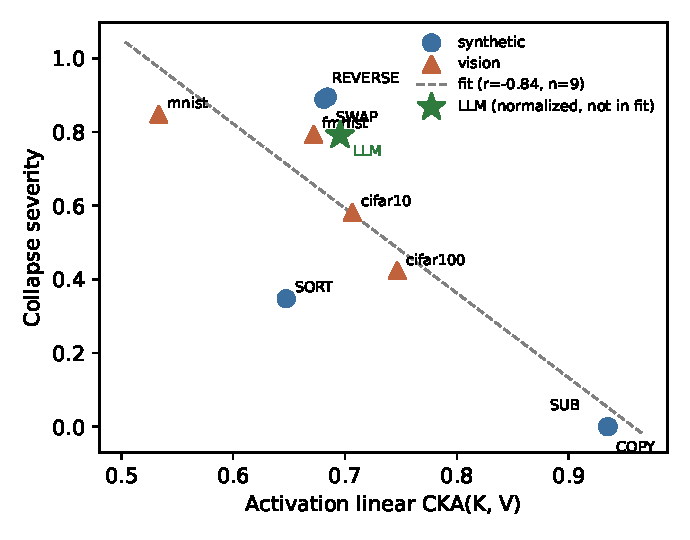
\includegraphics[width=0.62\textwidth]{../kv_cka_vs_collapse.pdf}
\caption{Activation-level linear CKA between a teacher's trained $K$ and $V$
projections vs.\ the accuracy drop under K=V surgery (averaged over \textsc{keep\_k}
and \textsc{keep\_v}), across all 5 synthetic tasks and 4 vision datasets.
Pearson $r = -0.84$ ($n=9$); see text for why we do not treat this as a validated
general predictor. The star marks the same measurement on the 300M-parameter
FineWeb-Edu teacher (CKA $=0.70$), with its $y$-coordinate a chance-normalized
log-loss severity in place of accuracy drop (Table~\ref{tab:llm} only gives
perplexity, which has no shared scale with accuracy): $(\ell_{\text{surgery}} -
\ell_{\text{teacher}}) / (\ln|V| - \ell_{\text{teacher}})$, where $\ell = \ln(\text{PPL})$
and $\ln|V|$ is the cross-entropy of a uniform predictor over the vocabulary --
the LM analogue of chance accuracy. Excluded from the fit regardless, since this is
a different derivation from the other 9 points' raw accuracy drop, not a directly
validated equivalent measure.}
\label{fig:cka}
\end{figure}

Across all 9 tasks, Figure~\ref{fig:cka} shows the predicted negative relationship:
\textsc{sub} and \textsc{copy} sit at the high-CKA ($0.93$--$0.94$) / zero-collapse
corner, while \textsc{reverse}, \textsc{sort}, \textsc{swap}, and every vision dataset
cluster at moderate CKA ($0.53$--$0.75$) with real collapse. This global correlation
is driven mainly by that between-group contrast -- pointwise tasks let $K$ and $V$
converge to near-identical functions with no cost, while every routing-dependent task
or dataset needs them to specialize at least somewhat.

\textbf{How much should $n=9$ and that between-group contrast worry us?} A fair
amount, and we report the numbers that say so rather than lead with the most
favorable one. Pearson's $r=-0.84$ ($p=0.005$) has a bootstrap 95\% confidence
interval of $[-0.98, -0.18]$ ($10^4$ resamples) -- consistent with a strong
relationship, but not tightly enough pinned down at $n=9$ to rule out a much weaker
one. Spearman's rank correlation, which does not reward the linear separation between
the pointwise cluster and everything else as heavily as Pearson does, is
$\rho=-0.56$ ($p=0.12$, not significant). And within each task-type group alone --
synthetic-only ($n=5$: $r=-0.82$, $p=0.09$) or vision-only ($n=4$: $r=-0.85$,
$p=0.15$) -- the correlation is directionally consistent with the global trend but
does not reach significance at these small within-group sample sizes. We therefore
do not treat CKA as a validated general predictor of collapse severity; it is a
useful, cheap diagnostic that lines up with the theory's qualitative prediction
across task types in this dataset, and the honest summary of the evidence for it is
weaker than the headline $r=-0.84$ makes it look.

What the correlation does \emph{not} explain is the ordering \emph{within} the vision
group. A natural hypothesis is that harder classification tasks force $K$ and $V$ to
specialize \emph{more} (lower CKA), which would explain why collapse gets worse from
MNIST to CIFAR-100. The data says the opposite: activation CKA \emph{rises}
monotonically with dataset difficulty (MNIST $0.53 \to$ FMNIST $0.67 \to$ CIFAR-10
$0.71 \to$ CIFAR-100 $0.75$), even as zero-shot collapse also gets worse. So whatever
drives increasing collapse severity across the vision datasets, it is not increasing
$K$--$V$ specialization -- CKA is doing the opposite of what that story requires. We do
not have an account for this and are not aware of one; we report it as an open
question rather than force a narrative onto it. One plausible (but unverified) reading
is that harder classification tasks lean more on the class token aggregating broad,
low-precision context from many patches -- a use of attention that Proposition~
\ref{prop:hull} restricts regardless of how similar $K$ and $V$ are -- so collapse
severity here may be tracking how much content-routing the task depends on, not how
specialized $K$ and $V$ happened to become. We leave testing that directly to future
work.

\textbf{Where in the network it happens.} Every model here has exactly two attention
layers, which lets us check layer-by-layer rather than only report the average. The
two domains show opposite trends. In the three routing-dependent synthetic tasks, CKA
is \emph{lower} in layer 0 than layer 1 (REVERSE $0.54\to0.82$; SORT $0.56\to0.74$;
SWAP $0.54\to0.83$): $K$ and $V$ specialize early and converge back toward redundancy
by the final layer. In vision the trend reverses -- CKA is high in layer 0 and drops in
layer 1, the layer immediately feeding the \textsc{cls} readout (MNIST
$0.74\to0.33$; FMNIST $0.77\to0.57$; CIFAR-10 $0.83\to0.58$; CIFAR-100
$0.79\to0.70$). Layer 0's CKA across the four vision datasets is not monotonic in
difficulty, but layer 1's is ($0.33 < 0.57 < 0.58 < 0.70$, i.e.\ MNIST $<$ FMNIST
$\lesssim$ CIFAR-10 $<$ CIFAR-100): the across-dataset trend already visible in
Figure~\ref{fig:cka} is carried almost entirely by the layer adjacent to the
classification readout. This sharpens, without resolving, the open question above --
whatever pushes harder vision datasets toward higher $K$--$V$ redundancy concentrates
at exactly the layer the class-token-aggregation account above would implicate, which
is consistent with that account without being evidence for it over any other.

\textbf{Robustness to the similarity measure.} All CKA numbers above use the linear
kernel. As a check that the pattern is not an artifact of that choice, we recomputed
every measurement with RBF-kernel CKA \cite{kornblith2019similarity} instead (median
pairwise-distance bandwidth; activations subsampled to 2000 tokens per layer for
tractability). The global correlation with collapse severity is essentially unchanged
($r=-0.87$ vs.\ $r=-0.84$ for linear CKA, $n=9$, both $p<0.01$), and the qualitative
pattern is preserved throughout, including the vision layer-1 ordering above. We have
not evaluated CCA- or mutual-information-based similarity measures; we have no reason
to expect a different qualitative story from them, but we have not checked, and leave
it to future work rather than claim it.

Weight-space cosine similarity between the raw $(W_k, b_k)$ and $(W_v, b_v)$
parameters, by contrast, is uninformative in every task (all values within $\pm 0.005$
of zero) -- as expected, since two linear maps can compute highly redundant
\emph{functions} while living in unrelated parameter bases; only the
representation-level (CKA) comparison is basis-invariant and captures functional
overlap.

\section{Discussion}
\label{sec:discussion}

Recovery is fast relative to training from scratch: most (task, surgery-mode)
configurations reach the from-scratch tied baseline within 1--5 epochs of
distillation against the QKV teacher, versus the 10--50 epochs used to train the
corresponding checkpoints from scratch, and \textsc{keep\_v}/\textsc{avg} on CIFAR are
within a point of that baseline by 10 epochs (Table~\ref{tab:vision}). One fact about
the surgery
is certain and worth stating plainly: it leaves every parameter \emph{except}
$c_{kv}$ already correctly tuned (Section~\ref{sec:setup}), so distillation is
searching for a single linear map rather than re-deriving the whole network. Whether
that alone accounts for the observed speed of recovery -- as opposed to, say, the KL
term against the teacher's soft logits doing more work than the search-space argument
suggests -- we have not verified, and we do not offer a convergence-rate account here.
\textsc{keep\_k} is the clear counter-case to any simple "small search space, therefore
fast" story: it starts from the same reduced parameter count as \textsc{keep\_v} and
\textsc{avg} but is consistently the slowest and least complete to recover
(Table~\ref{tab:vision}). Section~\ref{sec:mechanism}'s basis-mismatch account is more
consistent with this than Corollary~\ref{cor:content} as originally stated: distillation
is not restoring content that \textsc{keep\_k} discarded (a linear probe shows the
content was never gone), it is re-calibrating $c_{\text{proj}}$/MLP/head to a
representation in an unfamiliar basis -- a harder fitting problem than the search-space
argument alone would suggest. The same asymmetry survives the jump from the 1.6M-param
CIFAR ViT to a 389M-parameter language model trained from scratch on 10B tokens --
more than two orders of magnitude more parameters, and a far larger, qualitatively
different pretraining corpus (Table~\ref{tab:llm}): \textsc{keep\_k} is still the
worst zero-shot mode and the one left furthest from the tied ceiling after a fixed
distillation budget, which weighs against reading the vision-scale \textsc{keep\_k}
gap as an artifact of the vision ViT being too small or CIFAR too little data for
full re-calibration. The LLM's own content probe complicates this account rather than
simply extending it, though (Section~\ref{sec:empirical}): unlike the synthetic/vision
teachers, where $K$ and $V$ decoded token identity equally well, this teacher's $K$ is
measurably (if modestly) harder to decode than $V$ at every layer -- some genuine
content asymmetry may be present at this scale on top of the basis-mismatch effect,
not instead of it, and we do not have a clean way from the current evidence to
apportion \textsc{keep\_k}'s slow recovery between the two.

The K$\to$V alignment result (Section~\ref{sec:direct-tests}) sharpens what
"re-calibrating to an unfamiliar basis" means concretely: a full knowledge-distillation
pass updates every downstream parameter against a much richer training signal
(hard labels plus the teacher's soft logits, many epochs or hundreds of millions of
tokens), while the alignment correction updates \emph{nothing} downstream and is a
single closed-form linear or orthogonal fit on far less data. That such a cheap,
purely representational fix gets most of the way to \textsc{keep\_v} at every scale
we tested -- rather than distillation's slow, expensive re-calibration being
necessary in principle -- suggests the bulk of \textsc{keep\_k}'s deficit really is a
change-of-basis problem, small compared to what generic downstream re-training would
be needed for if the content itself were the missing piece. That distillation still
converges slower for \textsc{keep\_k} than for \textsc{keep\_v}/\textsc{avg} despite
the fix being this cheap in principle is itself informative: gradient descent
evidently does not find the closed-form correction directly, or finds it more slowly
than it finds whatever \textsc{keep\_v}/\textsc{avg} need, which we have not
investigated further.

\section{Related work}
\label{sec:related}

\textbf{Attention as constrained computation.} Tsai et al.~\cite{tsai2019kernel}
reframe self-attention generally as a kernel smoother: $y_i$ is a weighted average of
value vectors, with the softmax scores acting as a data-dependent kernel. That framing
already implies Proposition~\ref{prop:hull} as a special case once the vectors being
smoothed and the vectors used to produce the kernel weights are forced to be the same
object ($k=v$): the kernel-smoother view says the output lies in the convex hull of
whatever is being smoothed, and our contribution is narrower and
architecture-specific -- showing what that hull becomes, and why it is a genuine
bottleneck for some tasks and not others, exactly when $K=V$.

Two other lines of work probe different senses in which attention is ``limited,'' and
it is worth being precise about how ours differs from each. Dong et
al.~\cite{dong2021attention} show that stacked self-attention without skip connections
or MLPs collapses token representations to rank 1 doubly exponentially with depth -- a
degeneracy that compounds across many layers of attention interacting with each other.
Proposition~\ref{prop:hull}'s obstruction is unrelated to depth: it is a single-layer
statement about the span reachable by one attention block once $K=V$, holds regardless
of how many layers are stacked, and does not require removing the skip connections or
MLPs that Dong et al.\ show arrest their collapse (our checkpoints keep both
throughout). Raganato et al.~\cite{raganato2020fixed} show that replacing most encoder
attention heads with fixed, non-learned, position-based patterns barely hurts
translation quality -- i.e.\ the specific values of the attention weights $a_{ij}$ are
often not doing much specialized work. That is an empirical, training-time finding
about how much freedom the \emph{weights} need; ours is an architectural,
weight-independent statement about what the \emph{value space} can carry once $K=V$ --
Proposition~\ref{prop:hull} holds for every possible $a_{ij}$, learned or fixed, so the
limitation we describe is structural rather than something a better-trained or
differently-patterned attention could route around.

\textbf{Representational similarity.} Our CKA measurements follow Kornblith et
al.~\cite{kornblith2019similarity}, and the finding that raw weight-cosine similarity
is uninformative while activation-level CKA is not (Section~\ref{sec:empirical}) is
the expected consequence of CKA's basis invariance -- precisely the property it was
designed to have.

\textbf{Distillation.} Our recovery protocol (hard-label cross-entropy plus KL
divergence against soft teacher logits, $T=2$) follows Hinton et
al.~\cite{hinton2015distilling}. That paper, and most of the compression literature
built on it, uses distillation to shrink a model while preserving its architecture
class; here distillation instead repairs a capacity loss introduced by an
architectural edit made \emph{after} training (Section~\ref{sec:empirical}) -- a
different use of the same mechanism.

\textbf{KV-sharing architectures.} $K{=}V$ tying is a special case of a broader,
well-established family: multi-query attention shares $K/V$ across all heads
\cite{shazeer2019mqa}, and grouped-query attention shares them across groups of heads
\cite{ainslie2023gqa}; the base paper's own sweep includes exactly these variants
(GQA/MQA and their \texttt{Q}$\neq$\texttt{K=V} combinations) trained jointly from
scratch at 300M and 1.2B scale. None of that is new, and we do not claim otherwise.
What this note adds is orthogonal to the architecture choice itself: a mechanism for
\emph{why} imposing that same sharing structure \emph{after} independent training is a
qualitatively different operation from choosing it \emph{before} training starts, and
a cheap, testable account (Sections~\ref{sec:hull}, \ref{sec:mechanism}) of when the
difference is severe enough to matter. A reviewer's fair objection --
``$K$/$V$-sharing is not new; this is already standard in efficient attention'' -- is
correct about the architecture and, we think, orthogonal to what we are claiming about
the post-hoc/joint-training distinction.

\section{Conclusion}

The result we would ask a reader to take away is not ``$K=V$ is fundamentally
deficient'' -- \texttt{Q}$\neq$\texttt{K=V} trained jointly from scratch works fine
(the base paper's headline result), and two of our five synthetic tasks are entirely
untroubled by the surgery. The result is that \textbf{post-hoc merging of
independently-trained representations is a different operation from a joint
architectural constraint, with its own, separately characterizable failure mode}.
Joint training lets addressing and content pressures negotiate a shared
representation from the start; post-hoc merging imposes that constraint externally on
two representations that specialized apart under no such pressure, and Proposition~
\ref{prop:hull} gives a hard, narrow ceiling on what a single merged attention
sub-block -- not the whole network -- can then carry (Remark~\ref{rem:scope}).

Where that ceiling ends up mattering turned out to need more than the mechanism we
started with. Corollary~\ref{cor:content}'s original story -- $K$ addresses, $V$
carries content, so $K$ should be the less content-decodable of the two -- does not
survive a direct probe at synthetic/vision scale: $K$ and $V$ are equally linearly
decodable there (Section~\ref{sec:mechanism}). The same probe at LLM scale complicates
rather than confirms this: $K$ is measurably, if modestly, harder to decode than $V$
at every layer of the 300M-parameter model (Section~\ref{sec:empirical}), closer to
Corollary~\ref{cor:content} as originally stated -- so the content-loss and
basis-mismatch accounts may both be partially right, at different scales or in
different proportion, and we do not have the evidence to settle which. The evidence
at small scale is more consistent with a more specific, basis-mismatch account than
with Corollary~\ref{cor:content} as originally stated. Measured against a
random-projection baseline's own 5-seed spread rather than a single number,
\textsc{keep\_k} confers no detectable advantage over noise on most non-pointwise
tasks and is dramatically worse on one (Table~\ref{tab:randombaseline}), even though
its content is, by the same section's probe, fully present -- and, more decisively,
directly correcting $K$'s basis toward $V$'s with a learned linear or orthogonal map,
fit on held-out data with no retraining of anything downstream, closes the entire
\textsc{keep\_k} gap and matches or exceeds \textsc{keep\_v} at every scale we tested,
including the 300M-parameter LLM (Section~\ref{sec:direct-tests}). That last result is
a direct manipulation of the hypothesized mechanism, not an inference from indirect
signals, and is the strongest evidence in the note for reading \textsc{keep\_k}'s
failure as basis mismatch rather than content loss -- though a learned correction
working is consistent with the account without ruling out every alternative
explanation of the same result, so we still stop short of calling it established.
K--V activation
CKA is a useful and cheap diagnostic that tracks collapse severity across task types
in our data, but we do not oversell it as a validated general predictor: the
correlation is weaker under rank statistics than under Pearson's, is not separately
significant within either task-type group at our sample sizes, and runs in the
opposite direction of naive expectation \emph{within} the vision datasets for reasons
we do not have an account for (Section~\ref{sec:empirical}) -- three separate reasons
for a future study with more than $n=9$ tasks to revisit it. When the ceiling does
matter, a short knowledge-distillation pass against the original model is a
comparatively cheap and nearly-always-sufficient fix, with \textsc{keep\_k}
consistently the slowest to recover -- which the basis-mismatch account predicts,
since it is the mode with a genuinely unfamiliar representation to re-calibrate
against, not merely a smaller one.

\appendix

\section{LLM distillation curves}
\label{sec:appendix-llm-curves}

Table~\ref{tab:llm} reports only the zero-shot and final-budget perplexity for the
LLM-scale confirmation (Section~\ref{sec:empirical}); Figure~\ref{fig:llm-curves}
shows the full recovery trajectory for all three surgery modes, in the same spirit
as Figure~\ref{fig:curves} for the synthetic/vision runs.

\begin{figure}[h]
\centering
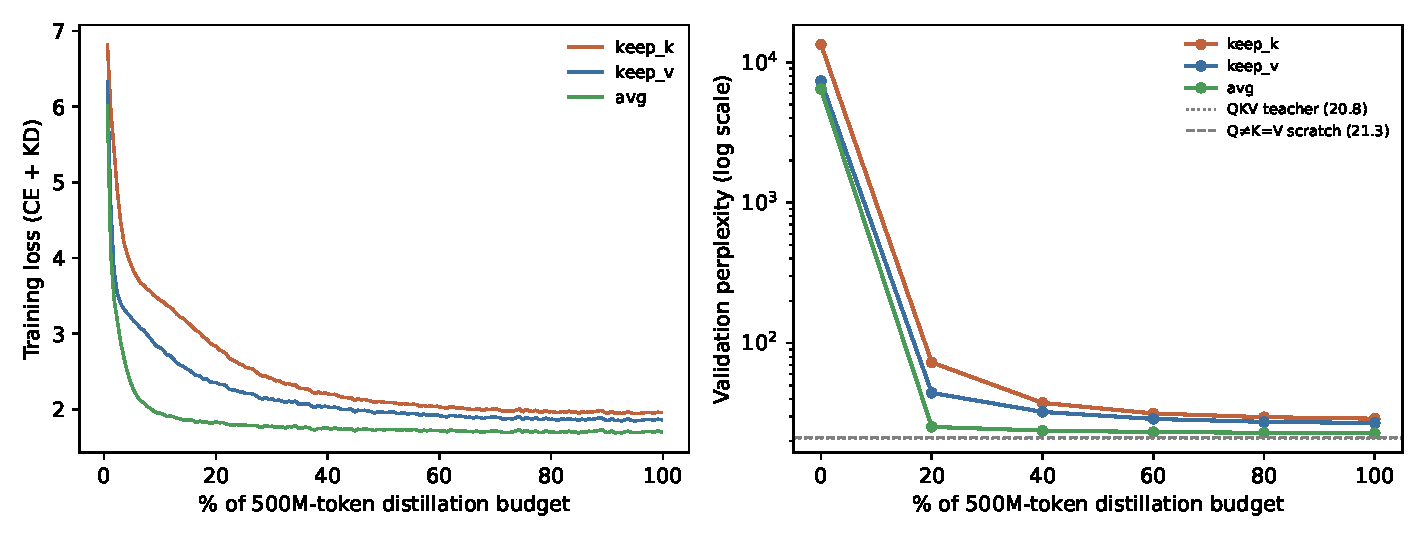
\includegraphics[width=\textwidth]{../distill_llm_curves.pdf}
\caption{Left: training loss (hard-label CE + KD against the QKV teacher's soft
logits) over the 500M-token distillation budget, parsed directly from the training
logs (\texttt{distill\_llm\_\{keep\_k,keep\_v,avg\}.log}). Right: validation
perplexity at the zero-shot point and each of the 5 evaluation checkpoints (log
scale, given the roughly three-orders-of-magnitude range from zero-shot collapse to
recovered perplexity), against the QKV teacher and from-scratch Q$\neq$K=V ceiling
(dotted/dashed reference lines). All three modes make most of their recovery in the
first 20\% of the budget and continue closing the gap to the ceiling gradually
thereafter; \textsc{avg} and \textsc{keep\_v} track each other closely throughout,
while \textsc{keep\_k} remains visibly separated from both at every checkpoint,
consistent with its persistent gap in Table~\ref{tab:llm} and the slower,
less-complete \textsc{keep\_k} recovery already seen at synthetic/vision scale
(Figure~\ref{fig:curves}).}
\label{fig:llm-curves}
\end{figure}

\begin{thebibliography}{9}
\bibitem{kayyam2025} A. Kayyam et al. \emph{Do Transformers Need Three Projections?}
ICML (poster), 2025.
\bibitem{kornblith2019similarity} S. Kornblith, M. Norouzi, H. Lee, G. Hinton.
\emph{Similarity of Neural Network Representations Revisited.} ICML, 2019.
\bibitem{hinton2015distilling} G. Hinton, O. Vinyals, J. Dean. \emph{Distilling the
Knowledge in a Neural Network.} arXiv:1503.02531, 2015.
\bibitem{tsai2019kernel} Y.-H. H. Tsai, S. Bai, M. Yamada, L.-P. Morency, R.
Salakhutdinov. \emph{Transformer Dissection: An Unified Understanding for
Transformer's Attention via the Lens of Kernel.} EMNLP, 2019.
\bibitem{dong2021attention} Y. Dong, J.-B. Cordonnier, A. Loukas. \emph{Attention Is
Not All You Need: Pure Attention Loses Rank Doubly Exponentially with Depth.} ICML,
2021.
\bibitem{raganato2020fixed} A. Raganato, Y. Scherrer, J. Tiedemann. \emph{Fixed
Encoder Self-Attention Patterns in Transformer-Based Machine Translation.} Findings
of EMNLP, 2020.
\bibitem{shazeer2019mqa} N. Shazeer. \emph{Fast Transformer Decoding: One Write-Head
is All You Need.} arXiv:1911.02150, 2019.
\bibitem{ainslie2023gqa} J. Ainslie, J. Lee-Thorp, M. de Jong, Y. Zemlyanskiy, F.
Lebr\'on, S. Sanghai. \emph{GQA: Training Generalized Multi-Query Transformer Models
from Multi-Head Checkpoints.} EMNLP, 2023.
\end{thebibliography}

\end{document}
